\documentclass{article}
\usepackage[utf8]{inputenc}
\usepackage[T1]{fontenc}
\usepackage[english, ngerman]{babel}

\usepackage{amsmath}
\usepackage{amssymb}

\usepackage{siunitx} %\si{ampere} or \SI{0.3}{\angstrom}
%\sisetup{per-mode=fraction}
%\sisetup{separate-untertainty=true}
\usepackage[version=3]{mhchem}

\usepackage[pdftex]{graphicx}

\usepackage{pdfpages}

\usepackage{listings}

\usepackage{placeins}%provides \FloatBarrier

%put in deckblatt
\begin{document}

%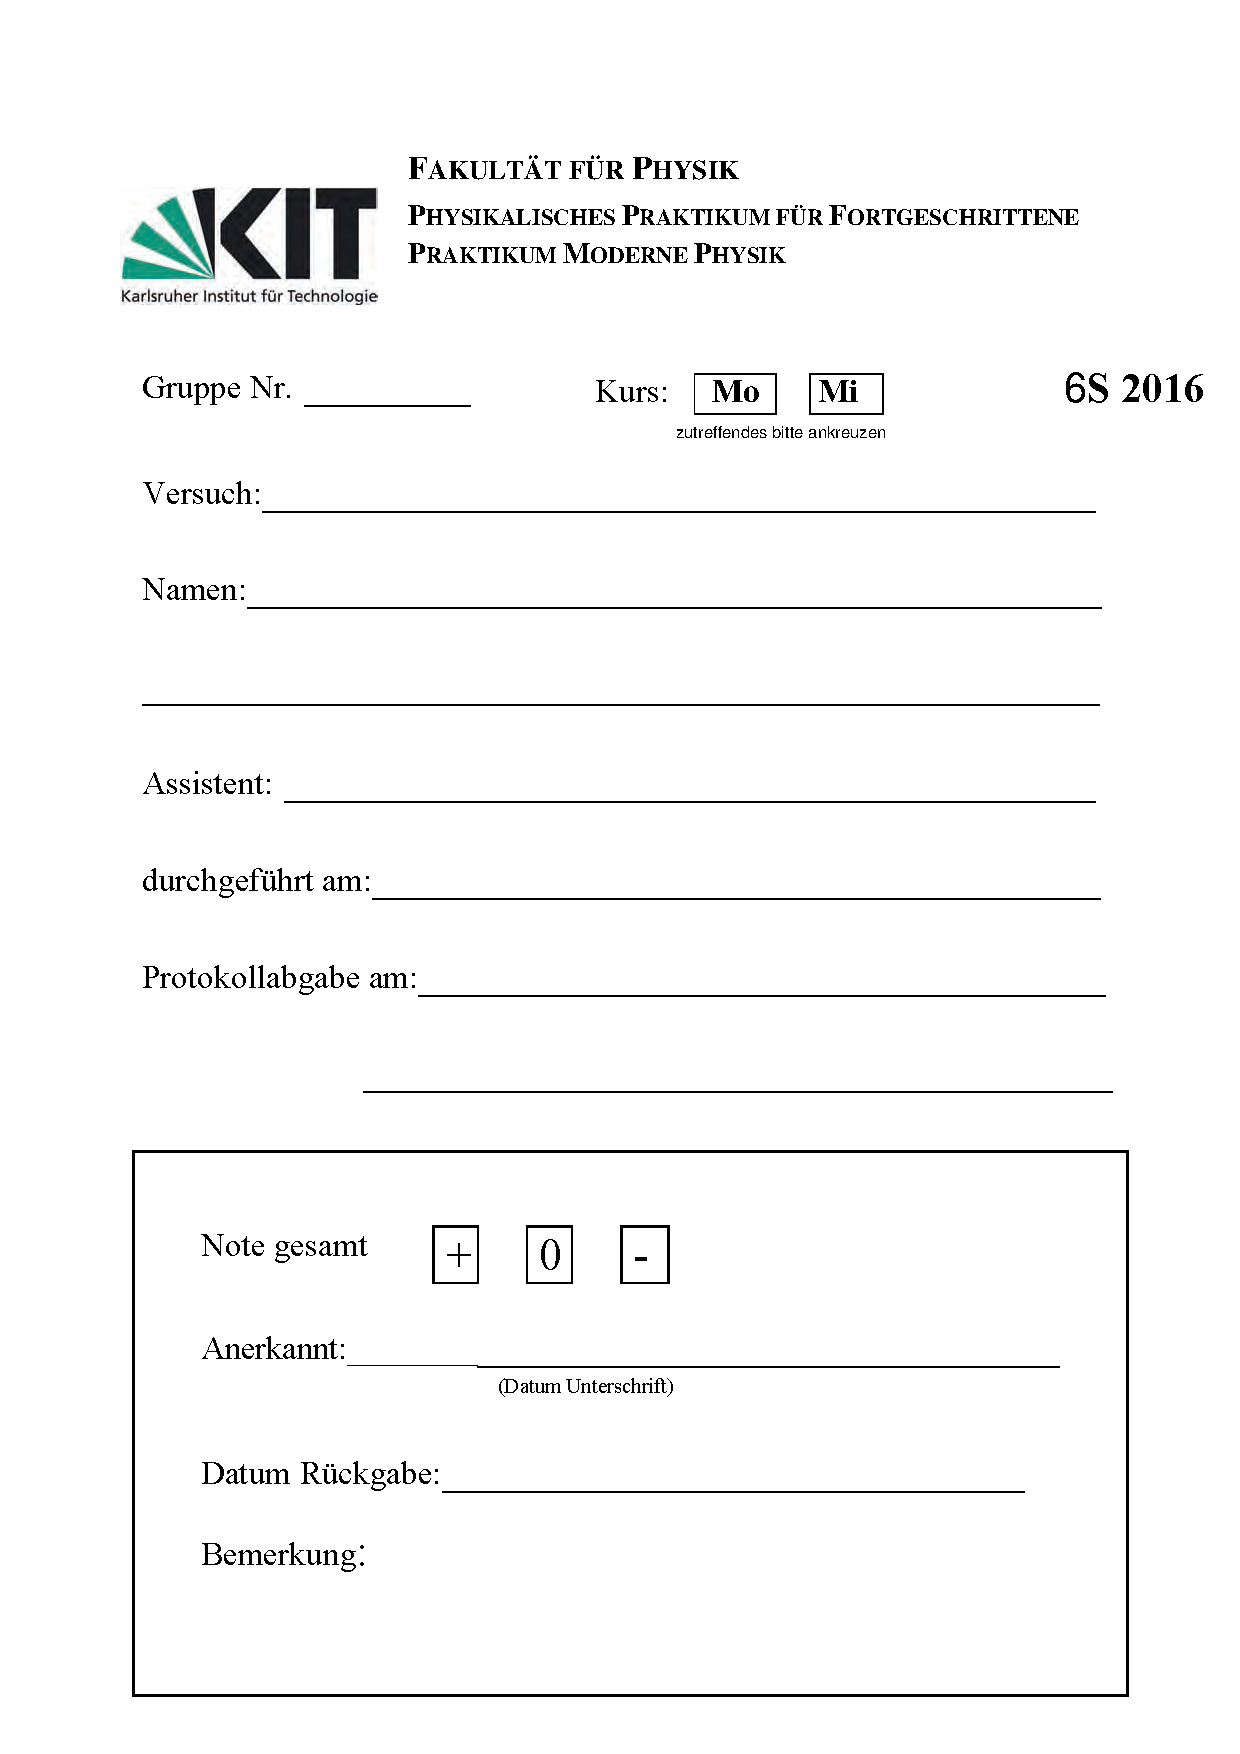
\includepdf[pages={1}]{DECKBLATT_SS16.pdf}

\section{Vorbereitung}
\subsection{Theoretischer Hintergrund}
Die Kapitel über den theoretischen Hintergrund, die Aufgaben und die Durchführung sind größtenteils übernommen und zusammengefasst aus der Staatsexamensarbeit "Der Quanten-Hall-Effekt im Fortgeschrittenenpraktikum"{} von Bianca Müller, welche im Dezember 1997 am Physikalischen Institut der Universität Karlsruhe (TH) angefertigt wurde. Hiervon abweichende Quellen sind im Text als Fußnote gekennzeichnet.
\subsubsection{Klassischer Halleffekt}
In einem stromduchflossenen Leiter bewegen sich Elektronen. Legt man senkrecht dazu ein B-Feld an, so erfahren diese eine Lorentz-Kraft senkrecht dazu. Im Gleichgewicht kompensieren sich die Lorentz-Kraft und das durch die Ablenkung entstehende E-Feld. Dann gilt:
$$\vec{F_L} = - \vec{F_E} $$
Der Hallkoeffizient ist definiert als:
$$ R_H = \frac{E_y}{j_x \cdot B} = \frac{1}{n e}$$
Bei endlicher Temperatur sind in Halbleitern nicht nur Elektronen sondern auch Defektelektronen, sog. Löcher, Ladungsträger. Für die Leitfähigkeit und den Hallkoeffizient gelten dann:
$$\sigma = ne\mu _n + pe\mu_p $$
$$R_H = \frac{p \mu _p ^{2} - n \mu _n ^{2}}{e(p\mu_p + n \mu _n)^{2}} $$
Hier sind $n,p$ die Ladungsträgerkonzentrationen und $\mu$ die jeweilige Beweglichkeiten.
\subsubsection{Verwendete Proben}
Die verwendeten Proben müssen ein 2D-Elektronengas bereitstellen. Das wird zum einen durch ein Silizium-MOSFET und zum anderen durch eine GaAs-GaAlAs-Heterostruktur realisiert.\\

Das Silizium-MOSFET besteht aus einem Block p-dotierten Siliziums mit einer Isolationsschicht darüber. Die Gate-Spannung $V_G$ wird angelegt an eine auf der anderen Seite befindlichen Aluminium-Schicht, sodass sich am Rand des Silizium-Blockes eine Inversionsschicht bildet, in der sich Elektronen in zwei Dimensionen bewegen können. Die Dichte der Ladungsträger kann hierbei gut über die Gate-Spannung eingestellt werden. Durch recht starke Streuung an Störstellen ist die Beweglichkeit der Elektronen jedoch gering. \\

In der GaAs-GaAlAs-Heterostruktur übernimmt die leicht p-dotierte GaAs-Schicht die Rolle des Silizium-Blockes. Durch Diffusion der überschüssigen Elektronen mit den Löchern an der Grenzfläche, werden erstere räumlich von den zugehörigen Störstellen getrennt, jedoch noch angezogen\footnote{R.E.Prange, S.M. Girvin,eds: The Quantum Hall Effect, Springer Verlag, New York, 1990}. Dadurch können diese sich in der Grenzfläche bewegen. 
\subsubsection{2DEG}
In einem 2D-Elektronengas, das wie oben beschrieben realisiert werden kann, ist eine Koordinate festgehalten. Legt man ein B-Feld senkrecht zur Stromflussrichtung an, so kommt es zum Quantenhalleffekt. Die Elektronen bewegen sich auf einer Spiralbahn senkrecht zur Oberfläche und bilden Landau-Niveaus. Diese sind entartet, sodass die Fermienergie sprunghaft steigt, wenn ein Niveau vollständig besetzt ist. Dadurch sind in der Hallspannung Plateaus mit steigendem B-Feld zu beobachten. \\
Die Leitfähigkeit längs einer Bewegungsrichtung des 2D-Elektronengases oszilliert mit steigendem B-Feld, da das oberste Energieband zum Teil höher als die Fermienergie liegt und dadurch geleert wird. Die abgegebene Energie erhöht die Streuung der Elektronen an Störstellen, was zu einer Änderung der Leitfähigkeit führt.
\subsubsection{Änderung der Temperatur und des Probenstromes}
Wird die Temperatur zu stark erhöht, so ist kein Quantenhalleffekt mehr erkennbar, da die Struktur des 2DEG nicht mehr gilt und höhere Landau-Niveaus nicht besetzt werden. Die Temperatur von flüssigem Stickstoff reicht hierzu nicht aus.\\
Bei Änderung des Probenstroms treten oben beschriebene Oszillationen der Leitfähigkeit auf.
\subsubsection{Zeeman-Aufspaltung}
Energieniveaus von Atomen spalten sich auf in einem Magnetfeld. Dieser Effekt ist bekannt als Zeeman-Effekt. In diesem Versuch spielt er keine Rolle. 
\newpage
\subsection{Durchführung}
Zunächst wird der Kryostat abgekühlt. Davor wird allerdings geprüft, ob die Probe korrekt eingebaut ist, da später nicht nachjustiert werden kann. \\
Dann werden die einzelnen Kammern in der Versuchsanordnung mit Helium gespült, bevor flüssiger Stickstoff eingefüllt wird. Der Widerstand der Spule und des Thermometers werden gemessen. \\
Dann wird der flüssige Stickstoff entfernt und das Dewar sowie der Probenraum wieder mit Helium gefüllt. Anschließend wird der Probenraum auf ca. 2 mbar evakuiert und das Dewar erneut gespült. Danach wird der Kryostat mit Helium gefüllt. Das geschieht wieder bei einem Druck von 2,0 mbar. Die Füllhöhe wird über Schwingungen eines Messstabes ermittelt. Erreicht dieser die Oberfläche des Bades, so steigt die Frequenz. \\
Abschließend werden der Widerstand der Spule und die Temperatur ermittelt. Die Spule sollte supraleitend sein, die Temeperatur sollte unter 4,2 K sein. Dann können die Messungen durchgeführt werden.
\subsection{Aufgaben}
Bei 4 K wird die Längs- und die Querspannung gemessen. \\
Durch verdampfen von flüssigem Helium wird die Probe auf 1,8 K abgekühlt. Bei einem Probenstrom von $10 \mu A$ wird das B-Feld auf 6 T hochgefahren und dabei die Längsspannung in 0.5 T schritten gemessen. Beim Herunterfahren des B-Feldes wird die Querspannung gemessen. Anschließend werden beide Spannungen bei einem Strom von $100 \mu A$ gemessen. Dann wird die Messapparatur ausgeschalten. \\

Zur Auswertung werden die Extrema der Längspannung bestimmt mit den dazugehörigen Magnetfeldstärken. \\
Die Quer- oder Hallspannung der Plateaus wird bestimmt und diese auch identifiziert. \\
Damit wird dann über den Hallkoeffizienten die Ladungsträgerkonzentration bestimmt, sowie die Feinstrukturkonstante $\alpha$. Hierfür gilt\footnote{K. von Klitzing, G.Dorda, M.Pepper: New Method for High-Accuracy Determination of the Fine-Structure Constant Based on Quantized Hall Resistance, Phys. Rev. Lett., Vol. 45, No.6, 1980, p.494}: 
$$R_H = \alpha ^{-1} \mu _0 c /2i $$
Hier ist i die Nummer des besetzten Energieniveaus. Abschließend wird noch mit Literaturwerten verglichen.

%\section{Versuchsaufbau}
%\input{./chap/assembly.tex}

%\section{Versuchsdurchführung}
%\input{./chap/execution.tex}

%\section{Auswertung}
%
\subsection{Probe A}
\subsubsection{Leitfähigkeit und Hall-Koeffizient}
%auswerteformeln und probendimensionen angeben

Leitfähigkeit und Hall-Koeffizient der Proben sind Temperaturabhängig.
Es gelten die folgenden Beziehungen:
$$R_H = \frac{U_{H} \cdot b}{ I \cdot B }$$
$$\sigma = \frac{l \cdot I}{b \cdot d \cdot U_{leit}}$$

wobei $l = 19 \text{mm}$, $b = 10 \text{mm}$ und $d = 1 \text{mm}$

\begin{figure}
\label{fig:R_H}
\centering
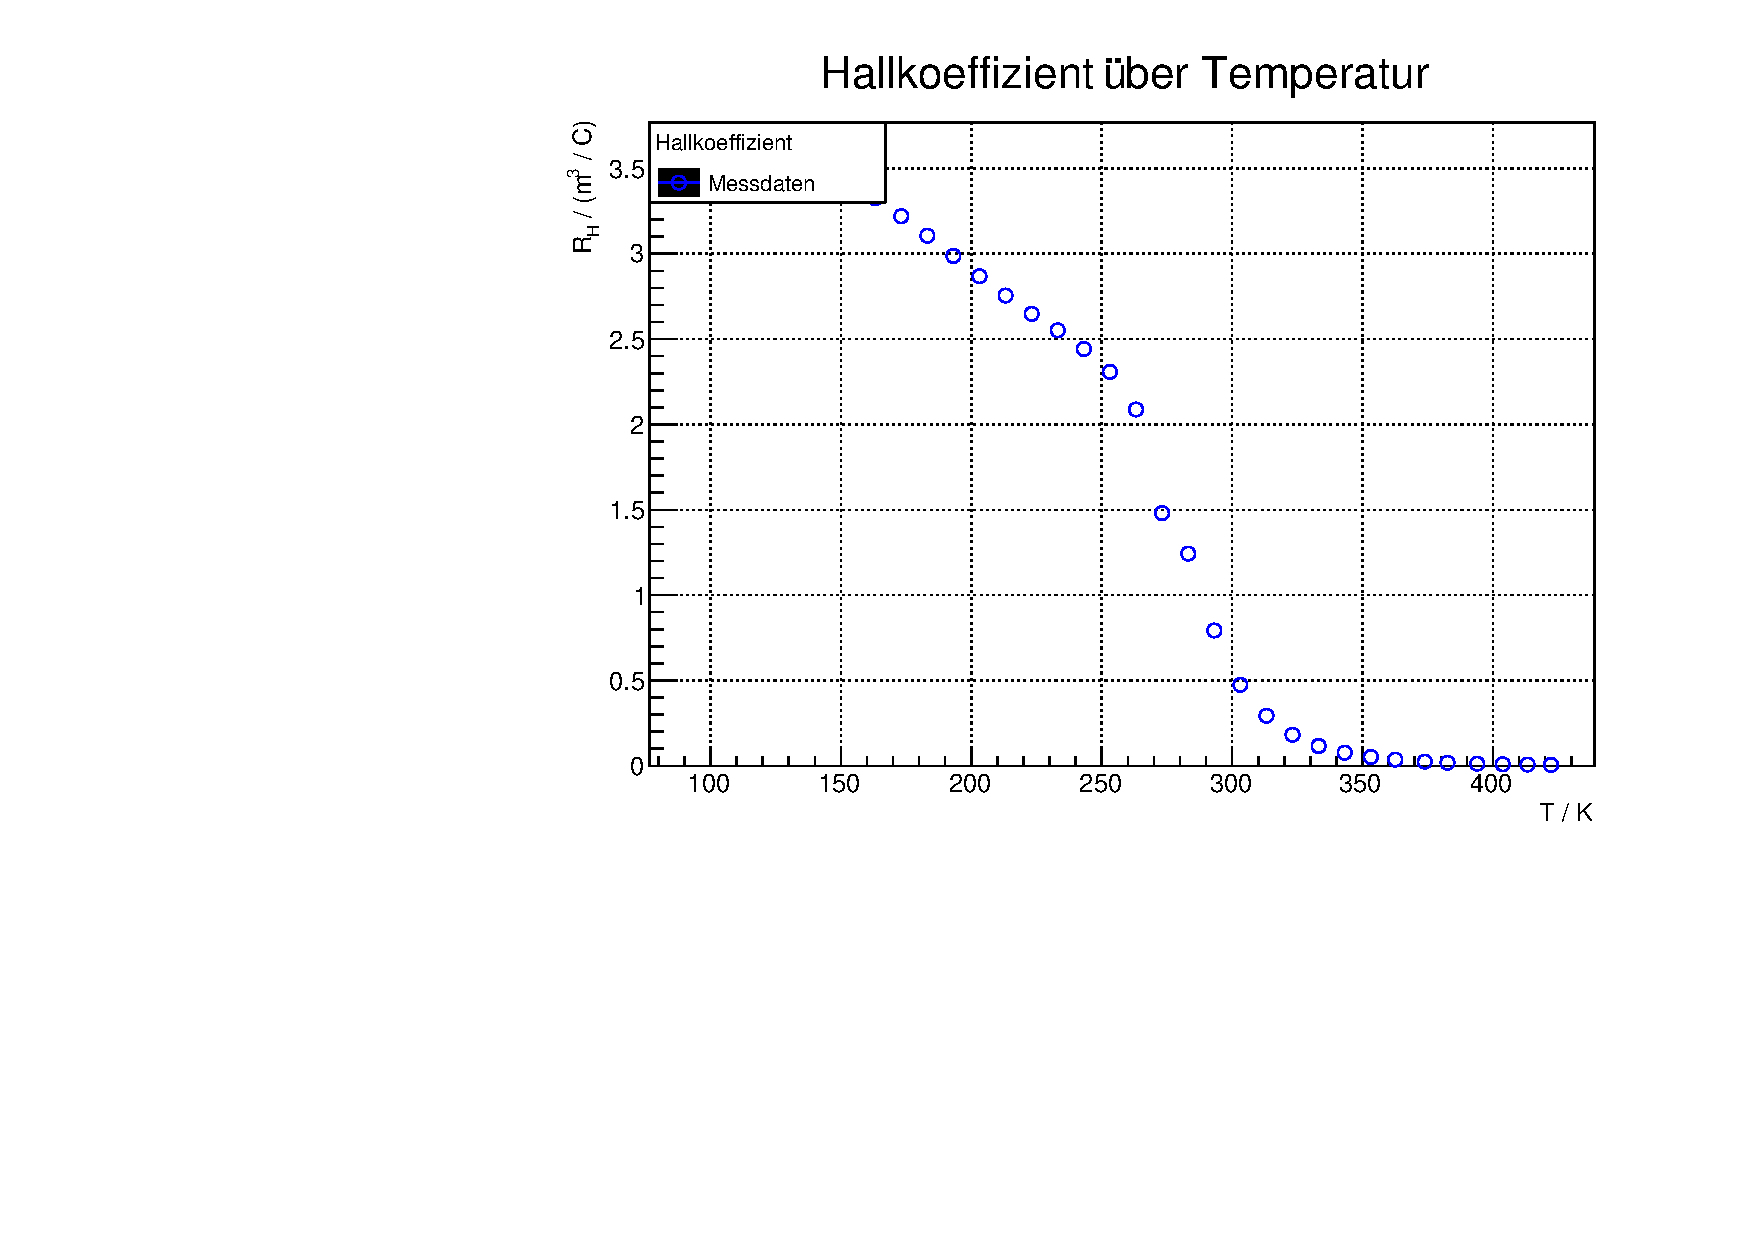
\includegraphics[scale = 0.5]{../data/A1R_h.pdf}
\caption{Hall Koeffizient von Probe A über der Temperatur}
\end{figure}

\begin{figure}
\label{fig:sigma}
\centering
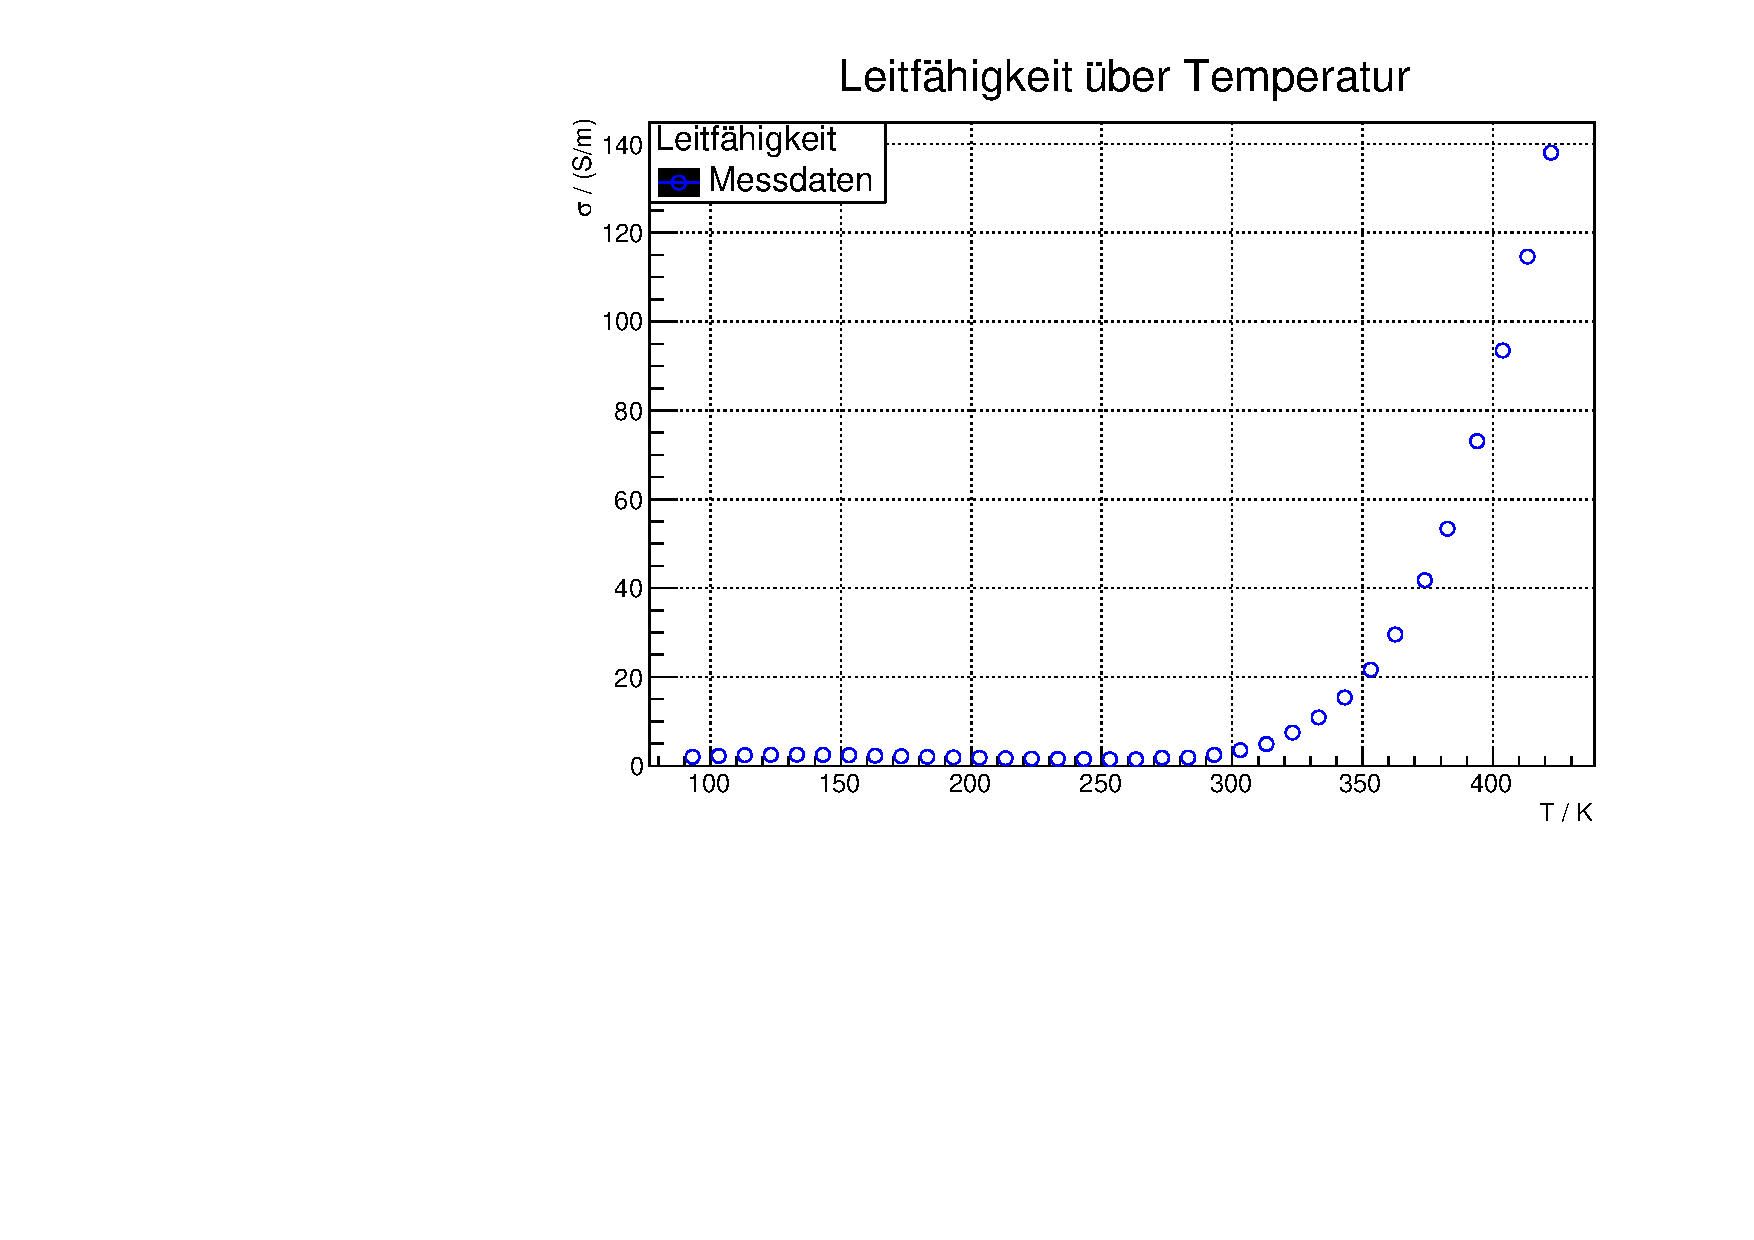
\includegraphics[scale = 0.5]{../data/A1sigma.pdf}
\caption{Leitfähigkeit von Probe A über der Temperatur}
\end{figure}


%formulas
%R_Hs = - UAH * b / (IAs * B ) * 0.001 # cubic meters / coulomb
%sigmas = l * IAs / (b * d * UAleit) # S / m # as should be

\subsubsection{Leitungsbereiche}
\FloatBarrier

Die Grenzetemperaturen für ex- und intrinsischen Leitungsbereich werden aus den Plots \ref{fig:leitex} und \ref{fig:leitin} abgelesen.
Der extrinische Bereich endet mit dem Plateau im inversen Hallkoeffizienten. Der intrinische Bereich beginnt ab dem linearen Bereich in $\sigma /cdot R_H}$.

%TODO pretty up the plots
%extrinsisch bis 270
%intrinsisch ab 310
\begin{figure}
\label{fig:leitex}
\centering
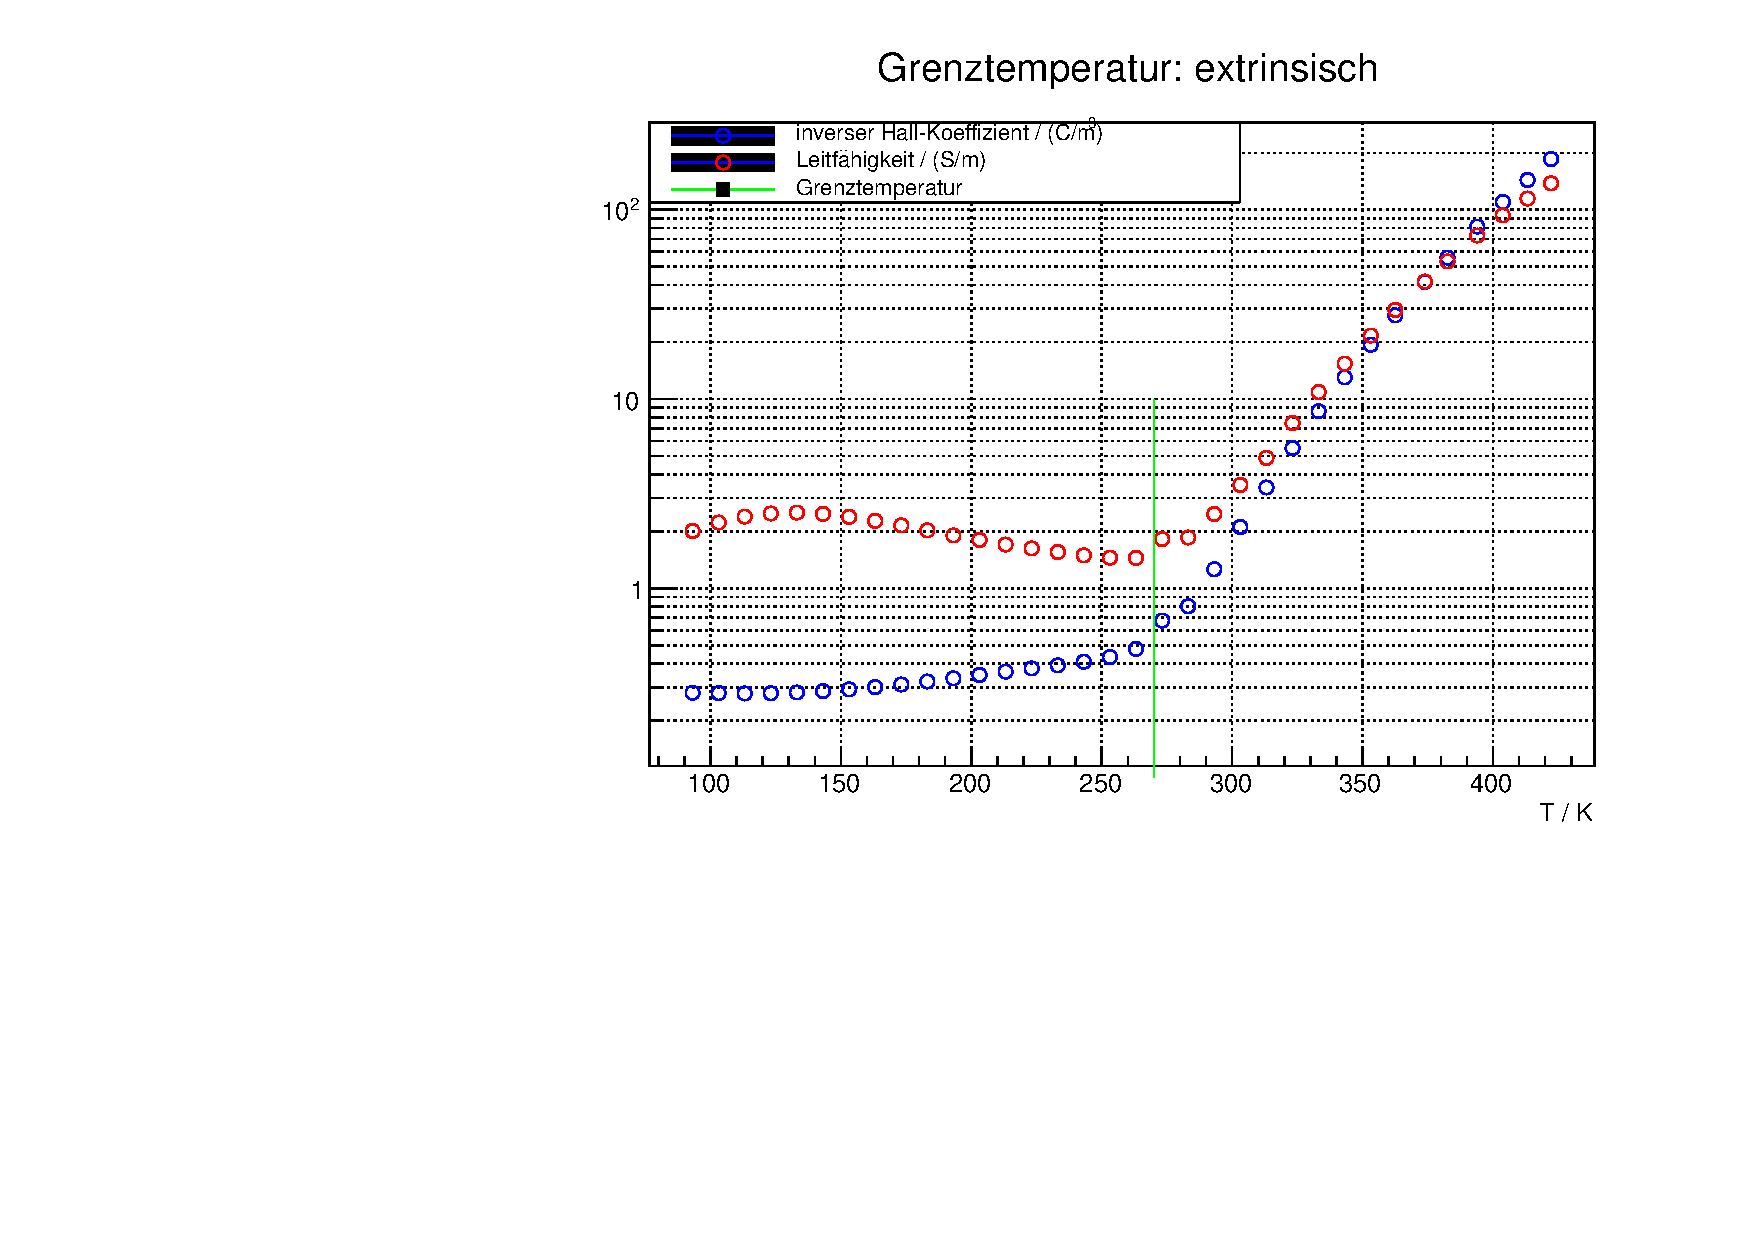
\includegraphics[scale = 0.5]{../data/A2ex.pdf}
\caption{Leitfähigkeit und inverser Hallkoeffizient}
\end{figure}

\begin{figure}
\label{fig:leitin}
\centering
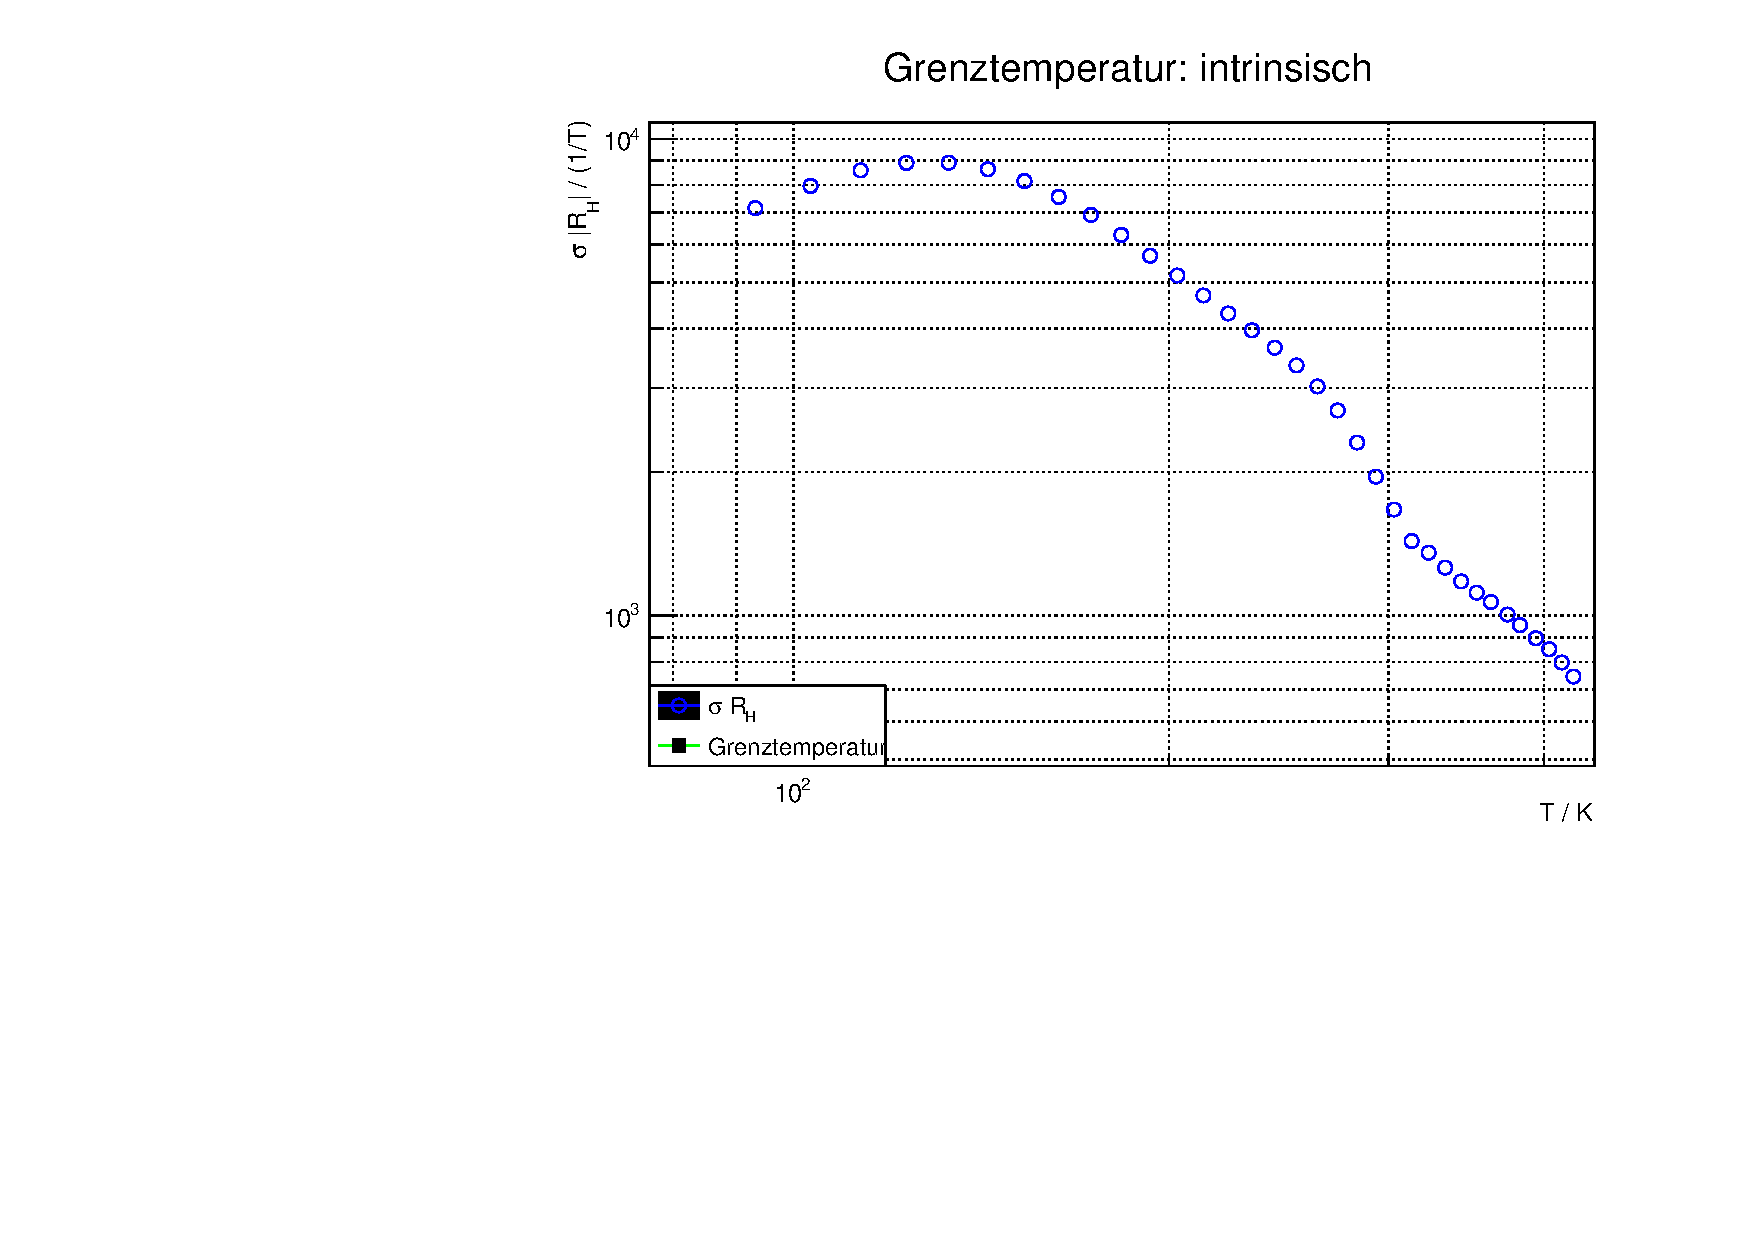
\includegraphics[scale = 0.5]{../data/A2in.pdf}
\caption{$\sigma /cdot R_H}$}
\end{figure}

\subsubsection{Leitungstyp}
\FloatBarrier

%Elektronenleitung???
%TODO thinking

\subsubsection{Intrinsische Ladungsträgerkonzentration}
\FloatBarrier

\begin{figure}
\label{fig:leitin}
\centering
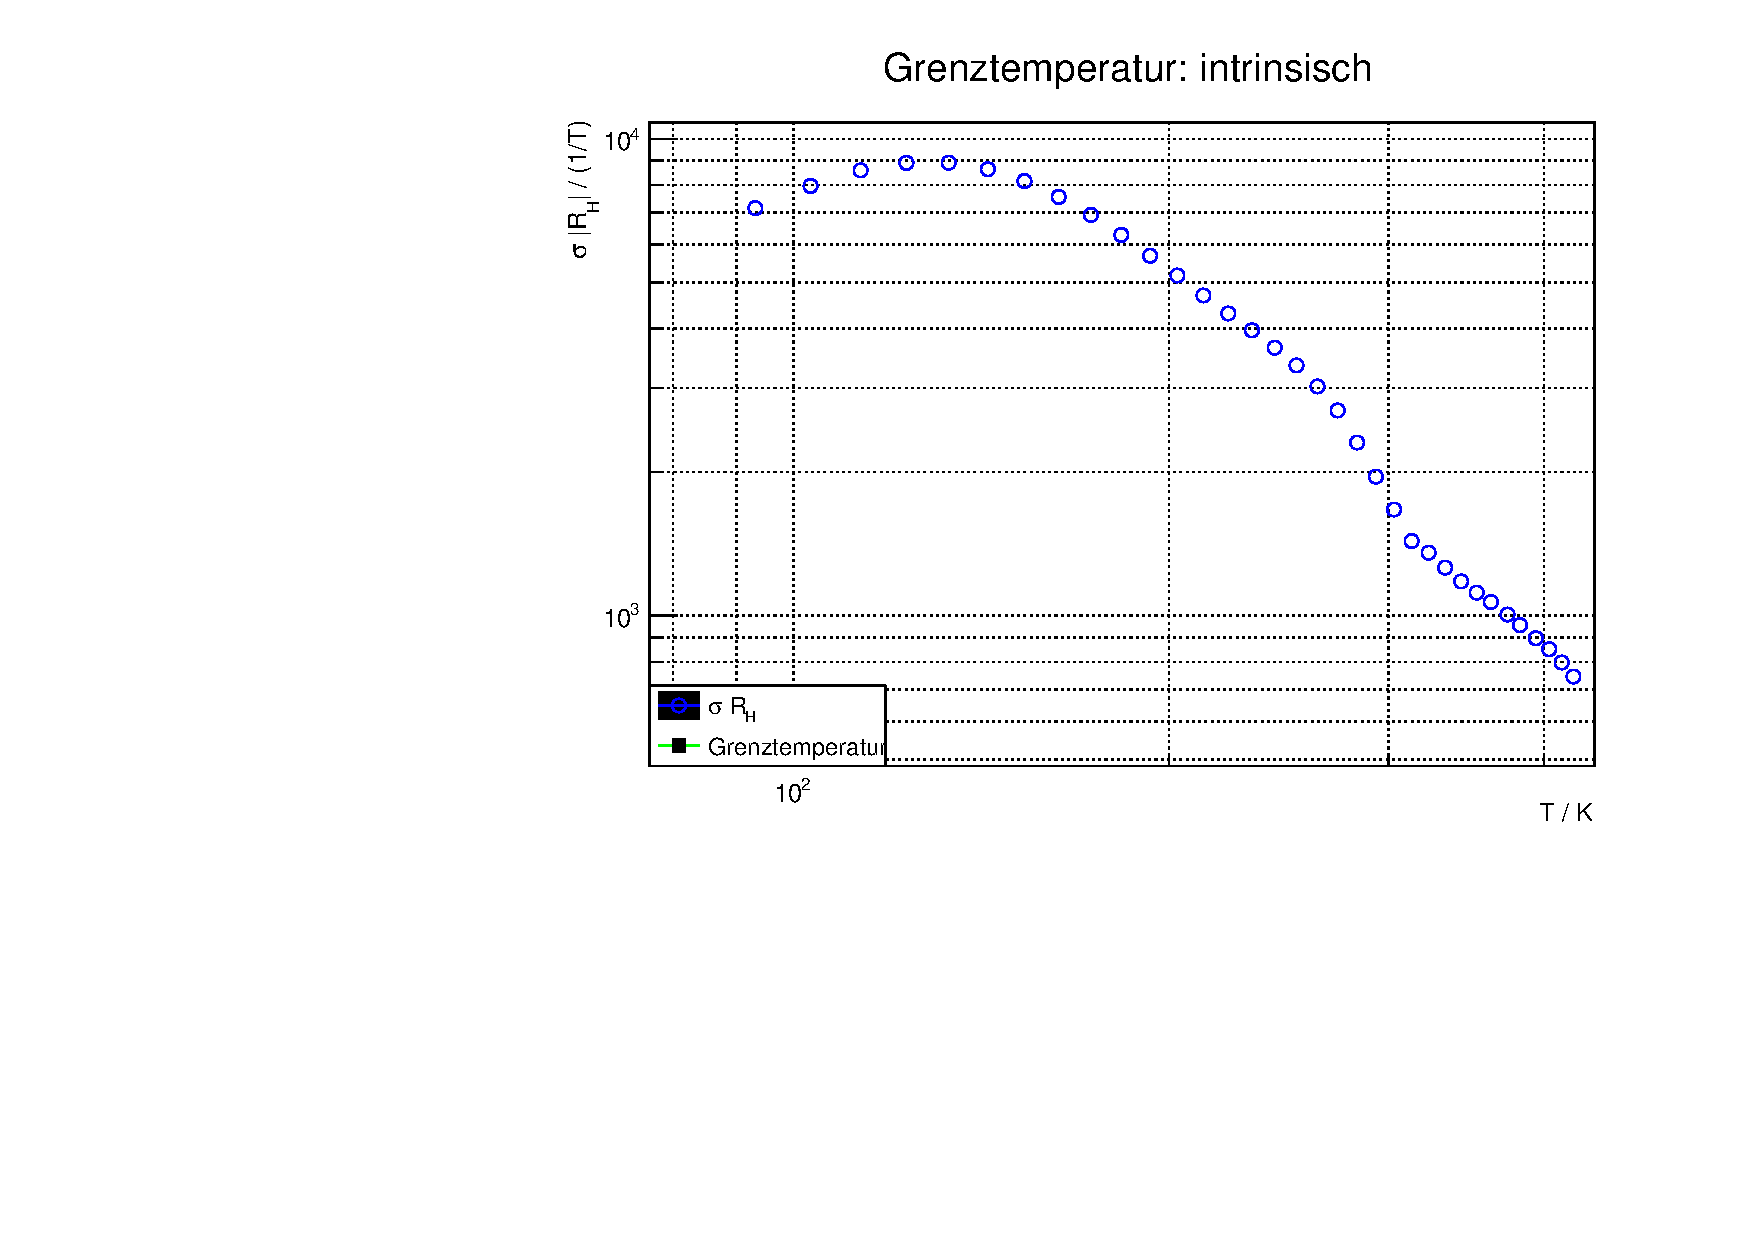
\includegraphics[scale = 0.5]{../data/A2in.pdf}
\caption{}
\end{figure}



\subsubsection{Arrhenius}
\FloatBarrier

%TODO oskar units
Aus dem Arrhenius-plot ergibt sich mit einem Chi2-Fit für die Bandlückenenergie und den y-Achsenabschnitt:
%$$y = -4467.87 \cdot x + 48.6613$$
$$\text{ln}(A) = 48.6613 \pm 0.0152968 $$
$$ - \frac{E_{G,0}}{2 \cdot k_B} = (-4467.87 \pm 5.55688 )  \text{K}$$
und damit:
$$E_{G,0} = 0.7695218869395287 \text{eV} $$

%y achsenabschnitt: 48.6613 +/- 0.0152968
%steigung: -4467.87 +/-5.55688
%E_G0 = -2 * kB * steigung

\subsubsection{Bandlücke bei 300K}
\FloatBarrier
Mit der Beziehung (44) aus der Vorbereitung gilt:
$$E_G(300K) = 0.6495218869395287 $$

\subsubsection{Intrinsische Ladungsträgerkonzentration bei 300K}
\FloatBarrier
Mit 
$$ n_i (T) = T^{3/2} /cdot A \cdot \exp^{- frac{E_{G,0}}{2 \cdot k_B }cdot T}}$$
ergibt sich:
$$n_i(300 \text{K} = 2.4049587717810924E+18 $$

\subsection{Probe B}
\subsubsection{Beweglichkeit}
\FloatBarrier

\subsubsection{Vergleich: Volumenhalbleiter und 2DEG}
\FloatBarrier

\subsection{Phononenstreuung}
\FloatBarrier




%appendix: original messprotokoll
%\Appendix
%\section{Messprotokoll}

\end{document}
